\PassOptionsToPackage{unicode=true}{hyperref} % options for packages loaded elsewhere
\PassOptionsToPackage{hyphens}{url}
\documentclass[9pt,ignorenonframetext,]{beamer}
\IfFileExists{pgfpages.sty}{\usepackage{pgfpages}}{}
\setbeamertemplate{caption}[numbered]
\setbeamertemplate{caption label separator}{: }
\setbeamercolor{caption name}{fg=normal text.fg}
\beamertemplatenavigationsymbolsempty
\usepackage{lmodern}
\usepackage{amssymb,amsmath}
\usepackage{ifxetex,ifluatex}
\usepackage{fixltx2e} % provides \textsubscript
\ifnum 0\ifxetex 1\fi\ifluatex 1\fi=0 % if pdftex
  \usepackage[T1]{fontenc}
  \usepackage[utf8]{inputenc}
\else % if luatex or xelatex
  \ifxetex
    \usepackage{mathspec}
  \else
    \usepackage{fontspec}
\fi
\defaultfontfeatures{Ligatures=TeX,Scale=MatchLowercase}







\fi

  \usetheme[]{metropolis}






% use upquote if available, for straight quotes in verbatim environments
\IfFileExists{upquote.sty}{\usepackage{upquote}}{}
% use microtype if available
\IfFileExists{microtype.sty}{%
  \usepackage{microtype}
  \UseMicrotypeSet[protrusion]{basicmath} % disable protrusion for tt fonts
}{}


\newif\ifbibliography
  \usepackage[style=abnt,]{biblatex}
      \addbibresource{citations.bib}
  

\hypersetup{
      pdftitle={Geoinformação na SPU/SC},
        pdfauthor={Luiz Fernando Palin Droubi},
          pdfborder={0 0 0},
    breaklinks=true}
%\urlstyle{same}  % Use monospace font for urls







% Prevent slide breaks in the middle of a paragraph:
\widowpenalties 1 10000
\raggedbottom

  \AtBeginPart{
    \let\insertpartnumber\relax
    \let\partname\relax
    \frame{\partpage}
  }
  \AtBeginSection{
    \ifbibliography
    \else
      \let\insertsectionnumber\relax
      \let\sectionname\relax
      \frame{\sectionpage}
    \fi
  }
  \AtBeginSubsection{
    \let\insertsubsectionnumber\relax
    \let\subsectionname\relax
    \frame{\subsectionpage}
  }



\setlength{\parindent}{0pt}
\setlength{\parskip}{6pt plus 2pt minus 1pt}
\setlength{\emergencystretch}{3em}  % prevent overfull lines
\providecommand{\tightlist}{%
  \setlength{\itemsep}{0pt}\setlength{\parskip}{0pt}}

  \setcounter{secnumdepth}{0}


  \usepackage[brazil]{babel}
  \usepackage{csquotes}

  \title[]{Geoinformação na SPU/SC}

  \subtitle{um curso prático}

  \author[
        Luiz Fernando Palin Droubi
    ]{Luiz Fernando Palin Droubi}

  \institute[
    ]{
    Superintendência do Patrimônio da União em Santa Catarina
    }

\date[
      \today
  ]{
      \today
        }

\begin{document}

% Hide progress bar and footline on titlepage
  \begin{frame}[plain]
  \titlepage
  \end{frame}


  \begin{frame}
  \tableofcontents[hideallsubsections]
  \end{frame}

\hypertarget{infraestrutura-de-dados-espaciais-ide}{%
\section{Infraestrutura de Dados Espaciais
(IDE)}\label{infraestrutura-de-dados-espaciais-ide}}

\begin{frame}{A IDE}
\protect\hypertarget{a-ide}{}

\begin{itemize}[<+->]
\tightlist
\item
  Desde a década de 90 cada país tem implementado uma IDE

  \begin{itemize}[<+->]
  \tightlist
  \item
    Argentina: \href{https://www.idera.gob.ar/}{IDERA}
  \item
    Uruguay:
    \href{https://www.gub.uy/infraestructura-datos-espaciales/}{IDEuy}
  \item
    Brasil: \href{https://www.inde.gov.br/}{INDE}
  \end{itemize}
\item
  Agenda 21 (UNCED)

  \begin{itemize}[<+->]
  \tightlist
  \item
    Em muitas áreas, a qualidade dos dados não é adequada
  \item
    Mesmo onde existem dados com qualidade, havia restrições de acesso
  \item
    Falta de padronização
  \end{itemize}
\end{itemize}

\end{frame}

\begin{frame}{Objetivos de uma IDE}
\protect\hypertarget{objetivos-de-uma-ide}{}

Segundo \textcite{INDE}:

\begin{itemize}[<+->]
\tightlist
\item
  Compartilhar IG (informação geográfica);
\item
  Incrementar a administração eletrônica no setor público;
\item
  Garantir aos cidadãos os direitos de acesso à IG pública para a tomada
  de decisões;
\item
  Incorporar a IG produzida pela iniciativa privada;
\item
  Harmonizar a IG disponibilizada, bem como registrar as características
  dessa IG;
\item
  Subsidiar a tomada de decisões de forma mais eficiente e eficaz.
\end{itemize}

\end{frame}

\begin{frame}{Componentes de uma IDE}
\protect\hypertarget{componentes-de-uma-ide}{}

\begin{figure}[H]

{\centering 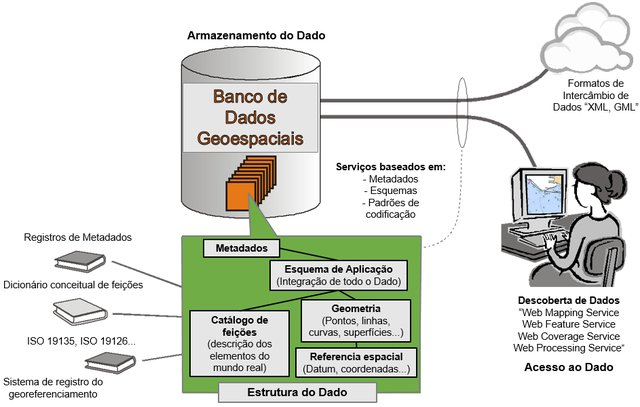
\includegraphics[width=0.7\linewidth]{images/Figura-2-Componentes-principais-de-uma-IDE_W640} 

}

\caption{Componentes de uma IDE. Fonte: \textcite{IDEM}.}\label{fig:unnamed-chunk-1}
\end{figure}

\end{frame}

\hypertarget{infraestrutura-de-dados-espaciais-no-brasil-inde}{%
\section{Infraestrutura de Dados Espaciais no Brasil
(INDE)}\label{infraestrutura-de-dados-espaciais-no-brasil-inde}}

\begin{frame}{A INDE}
\protect\hypertarget{a-inde}{}

\begin{itemize}
\item
  Marco legal da INDE: Decreto 6.666/08
\item
  Definição:
\end{itemize}

\begin{quote}
conjunto integrado de tecnologias; políticas; mecanismos e procedimentos
de coordenação e monitoramento; padrões e acordos, necessário para
facilitar e ordenar a geração, o armazenamento, o acesso, o
compartilhamento, a disseminação e o uso dos dados geoespaciais de
origem federal, estadual, distrital e municipal \autocite{INDE}.
\end{quote}

\end{frame}

\begin{frame}{Componentes da INDE}
\protect\hypertarget{componentes-da-inde}{}

\begin{center}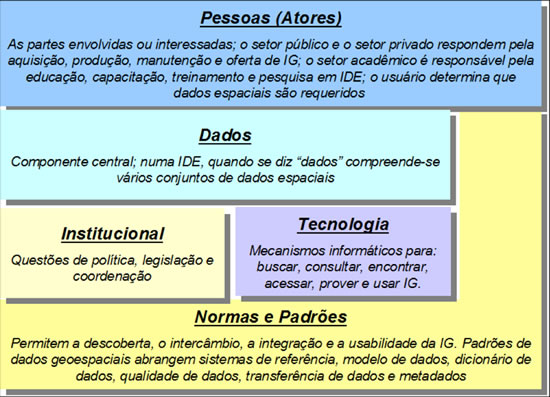
\includegraphics[width=0.7\linewidth]{images/Compenentes_INDE_2} \end{center}

\end{frame}

\begin{frame}{INDEM?}
\protect\hypertarget{indem}{}

\begin{itemize}[<+->]
\tightlist
\item
  \textcite{IDEM}
\end{itemize}

\begin{figure}[H]

{\centering 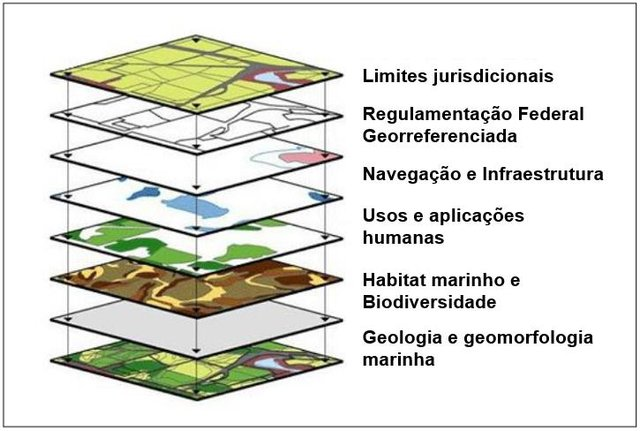
\includegraphics[width=0.7\linewidth]{images/Figura-4-Exemplo-da-organizacao-dos-temas-de-uma-IDEM_W640} 

}

\caption{Organização temática (IDEM). Fonte: \textcite{IDEM}.}\label{fig:unnamed-chunk-3}
\end{figure}

\end{frame}

\begin{frame}{Desafio SPU}
\protect\hypertarget{desafio-spu}{}

\begin{figure}[H]

{\centering 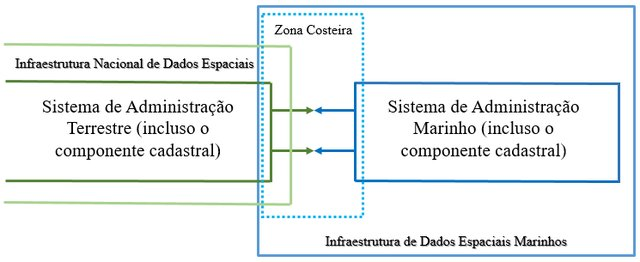
\includegraphics[width=0.7\linewidth]{images/Figura-3-Combinacao-entre-os-sistemas-de-gerenciamento-terrestre-e-marinho_W640} 

}

\caption{Combinação entre sistemas terrestre e marinho. Fonte: \textcite{IDEM}.}\label{fig:unnamed-chunk-4}
\end{figure}

\end{frame}

\hypertarget{armazenamento-de-informauxe7uxf5es-geogruxe1ficas}{%
\section{Armazenamento de Informações
Geográficas}\label{armazenamento-de-informauxe7uxf5es-geogruxe1ficas}}

\hypertarget{sistemas-de-referuxeancia}{%
\section{Sistemas de Referência}\label{sistemas-de-referuxeancia}}

\begin{frame}{A terra não é redonda}
\protect\hypertarget{a-terra-nuxe3o-uxe9-redonda}{}

\begin{block}{Geóide}

\begin{figure}[H]

{\centering 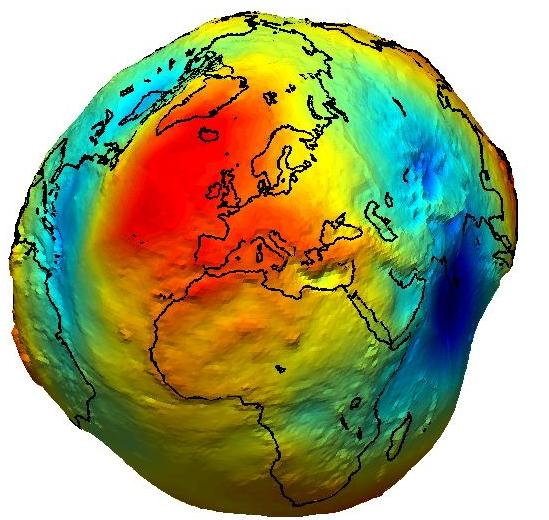
\includegraphics[width=0.65\linewidth]{images/geoide} 

}

\caption{Geóide.}\label{fig:unnamed-chunk-5}
\end{figure}

\end{block}

\end{frame}

\begin{frame}{A terra não é redonda}
\protect\hypertarget{a-terra-nuxe3o-uxe9-redonda-1}{}

\begin{block}{Elipsóide}

\begin{figure}[H]

{\centering 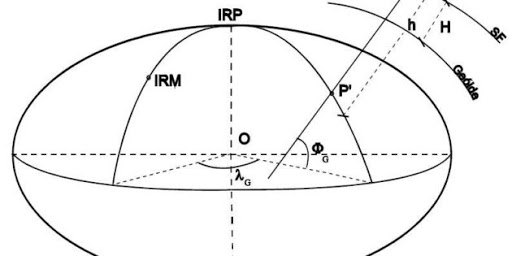
\includegraphics[width=0.7\linewidth]{images/elipsoide} 

}

\caption{Parâmetros de um elipsóide.}\label{fig:unnamed-chunk-6}
\end{figure}

O elipsoide é uma superfície que tem um modelo muito mais simples que o
geóide, e pode ser definida por um número bem menor de parâmetros.

\end{block}

\end{frame}

\begin{frame}[t]{Sistemas de referência ou \emph{datum}}
\protect\hypertarget{sistemas-de-referuxeancia-ou-datum}{}

\begin{itemize}[<+->]
\tightlist
\item
  Importância da adoção de um \emph{datum}
\end{itemize}

\begin{figure}[H]

{\centering 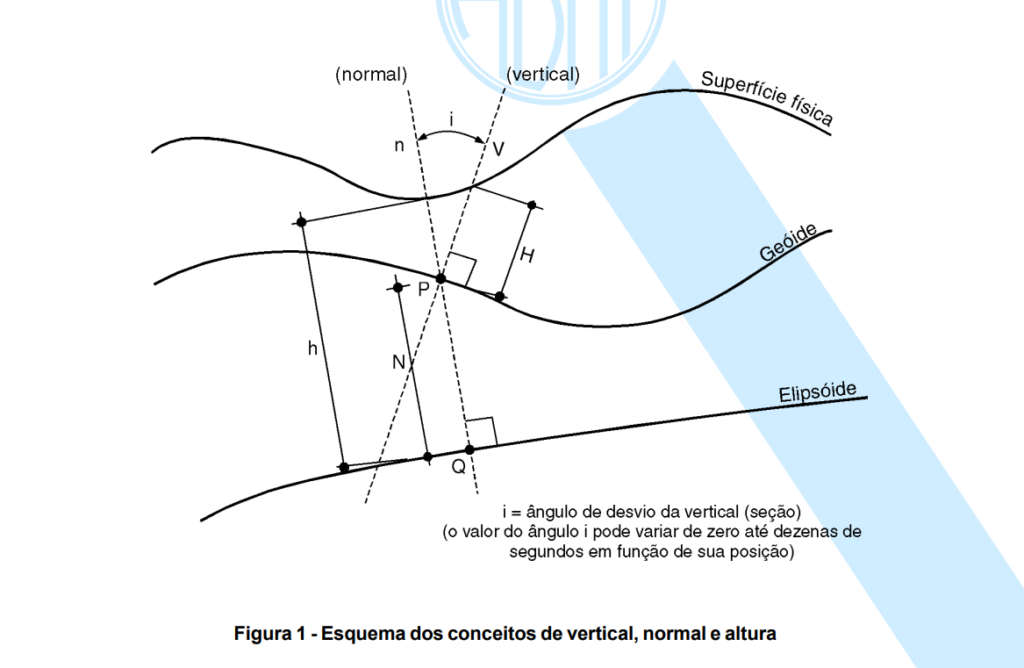
\includegraphics[width=0.5\linewidth]{images/nbr-14.166-datum-elipsoide-1024x668} 

}

\caption{Amarração entre as superfícies.}\label{fig:unnamed-chunk-7}
\end{figure}

\begin{itemize}[<+->]
\tightlist
\item
  São compostos de:

  \begin{itemize}[<+->]
  \tightlist
  \item
    Um ponto de amarração
  \item
    Um norte (orientação)
  \item
    Um elipsóide
  \end{itemize}
\end{itemize}

\end{frame}

\begin{frame}{Ilustração}
\protect\hypertarget{ilustrauxe7uxe3o}{}

\begin{figure}[H]

{\centering 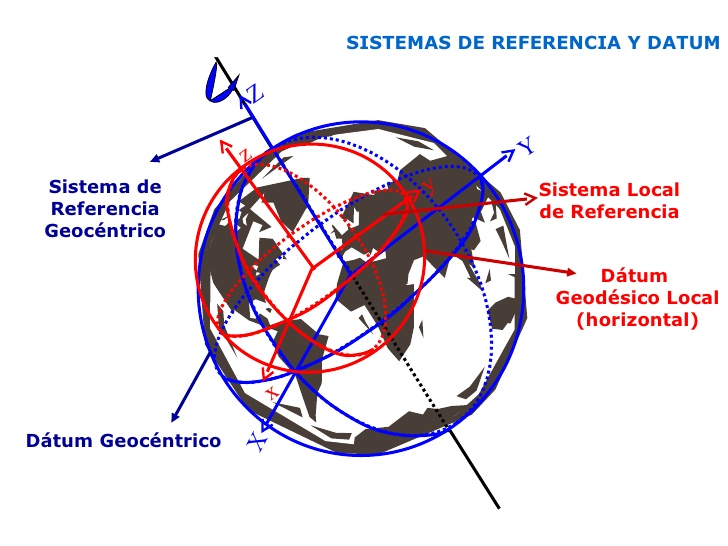
\includegraphics[width=0.7\linewidth]{images/sistema-de-referencia} 

}

\caption{Sistemas de Referências global e local.}\label{fig:unnamed-chunk-8}
\end{figure}

\end{frame}

\begin{frame}{SAD-69 vs.~SIRGAS2000}
\protect\hypertarget{sad-69-vs.-sirgas2000}{}

\begin{figure}[H]

{\centering 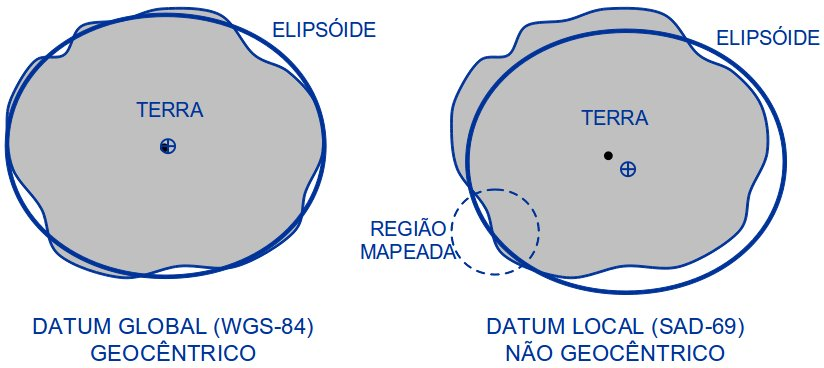
\includegraphics[width=0.7\linewidth]{images/sad-69-e-sirgas-WGS-84} 

}

\caption{Diferença entre o elipsóide do SIRGAS2000 e do SAD-69}\label{fig:unnamed-chunk-9}
\end{figure}

\end{frame}

\hypertarget{projeuxe7uxf5es}{%
\section{Projeções}\label{projeuxe7uxf5es}}

\begin{frame}[plain]{Projeções}
\protect\hypertarget{projeuxe7uxf5es-1}{}

\begin{figure}[H]

{\centering 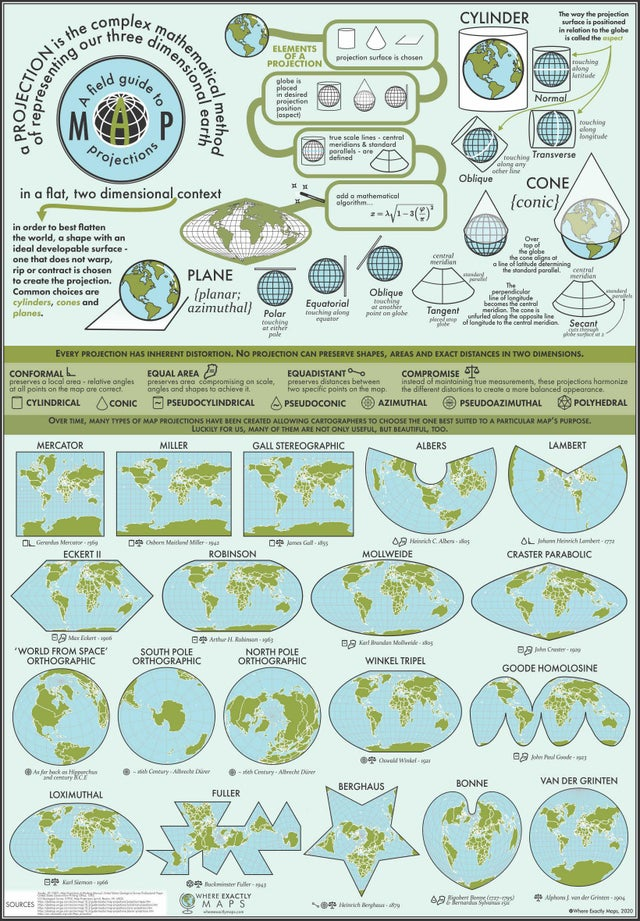
\includegraphics[width=1\linewidth]{images/projecoes} 

}

\caption{Projeções cartográficas.}\label{fig:unnamed-chunk-10}
\end{figure}

\end{frame}

\begin{frame}{Na prática}
\protect\hypertarget{na-pruxe1tica}{}

\begin{itemize}[<+->]
\tightlist
\item
  Código EPSG é atribuído a cada SRS.
\end{itemize}

\begin{itemize}[<+->]
\tightlist
\item
  Com as chegadas dos WebMapas 3D, projeções cartográficas praticamente
  perdem o sentido.
\end{itemize}

\begin{itemize}[<+->]
\tightlist
\item
  Mesmo nos WebMapas 2D atuais, já existe um padrão, que é a utilização
  da projeção Spherical Mercator
  (\href{http://epsg.io/3857}{EPSG:3857}).
\end{itemize}

\begin{itemize}[<+->]
\tightlist
\item
  Os dados são armazenados \emph{prioritariamente} em WGS-84
  (\href{http://epsg.io/4326}{EPSG:4326}), o padrão do formato
  \emph{geojson}, que tem se consolidado como um dos formatos mais
  utilizados, devido ao avança dos webmapas.
\end{itemize}

\end{frame}

\hypertarget{webgis}{%
\section{WebGIS}\label{webgis}}

\begin{frame}{Tecnologias}
\protect\hypertarget{tecnologias}{}

\begin{figure}[H]

{\centering 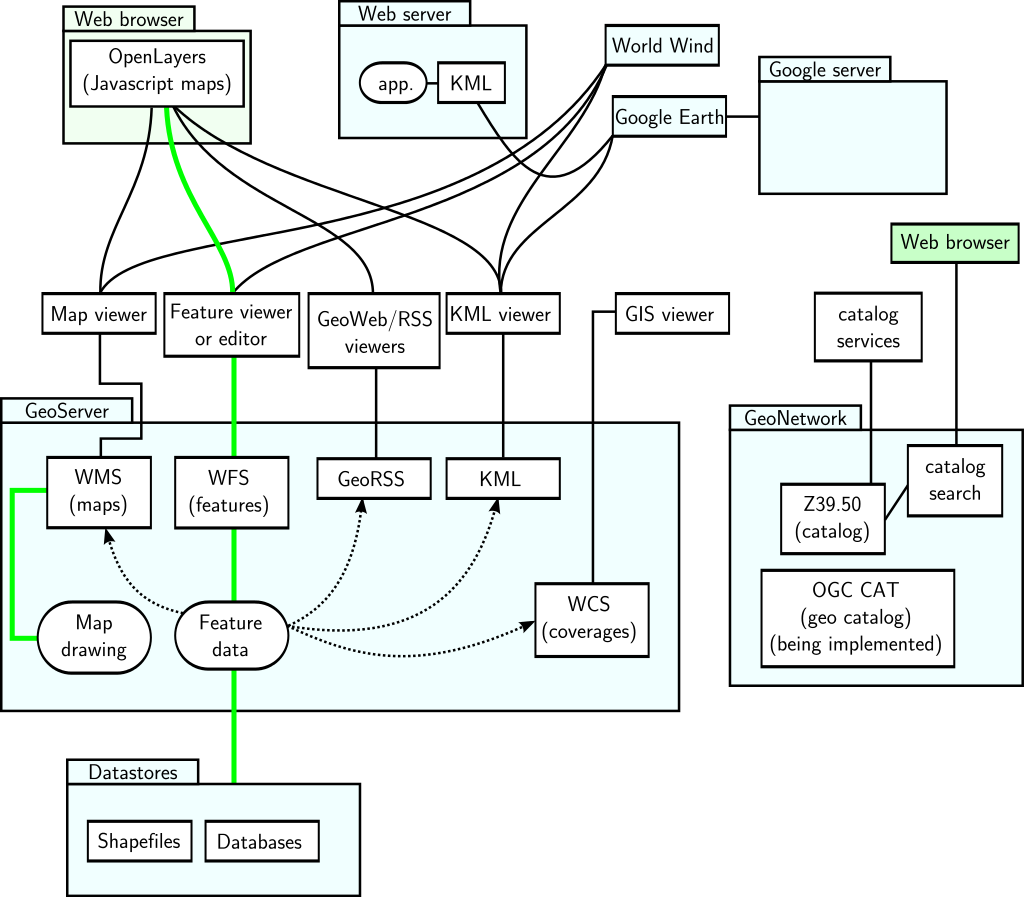
\includegraphics[width=0.7\linewidth]{images/GeoServer_GeoNetwork_with_web_app.svg} 

}

\caption{Tecnologia para confecção de WebMapas.}\label{fig:unnamed-chunk-11}
\end{figure}

\end{frame}

\begin{frame}[t]{Visualizadores de dados espaciais}
\protect\hypertarget{visualizadores-de-dados-espaciais}{}

\begin{itemize}[<+->]
\tightlist
\item
  Geovisualizadores

  \begin{itemize}[<+->]
  \tightlist
  \item
    \href{https://visualizador.inde.gov.br/}{INDE}
  \item
    \href{https://mapa.idera.gob.ar/}{IDERA}
  \item
    \href{https://www.gub.uy/infraestructura-datos-espaciales/publico/visualizador}{IDEuy}
  \item
    \href{http://www.catastro.cl/}{Chile (bens nacionais)}
  \item
    \href{https://idecor.cba.gov.ar/}{IDECor}
  \item
    \href{http://www.idesp.sp.gov.br/Visualizador}{IDE-SP}
  \item
    IDE-SPU?
  \end{itemize}
\end{itemize}

\end{frame}

\hypertarget{spuviz}{%
\section{SPUViz}\label{spuviz}}

\begin{frame}{SPUViz}
\protect\hypertarget{spuviz-1}{}

\begin{figure}[H]

{\centering 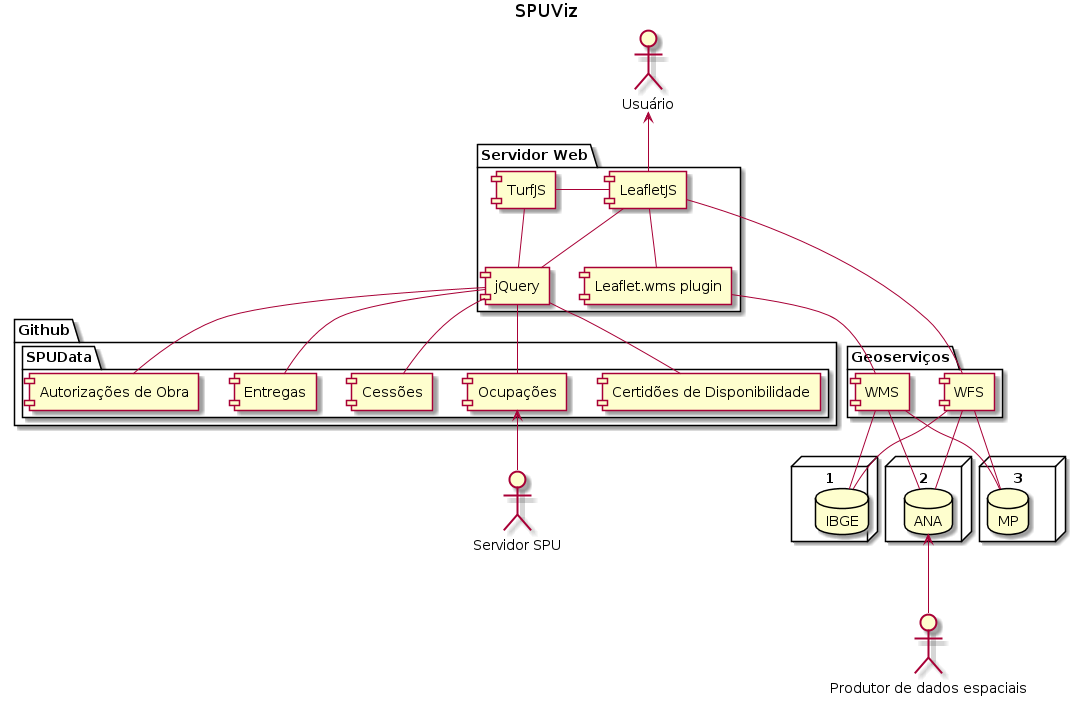
\includegraphics[width=0.8\linewidth]{images/modeloConceitual} 

}

\caption{Modelo Conceitual - Atual}\label{fig:unnamed-chunk-12}
\end{figure}

\end{frame}

\begin{frame}{SPUViz (futuro)}
\protect\hypertarget{spuviz-futuro}{}

\begin{figure}[H]

{\centering 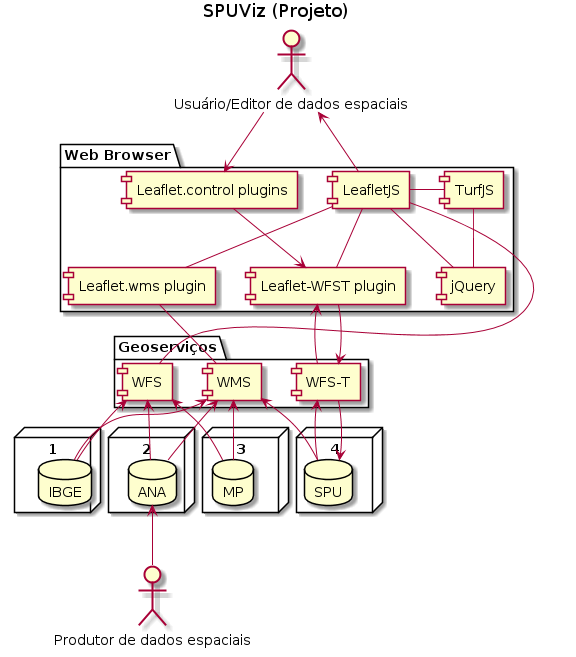
\includegraphics[width=0.6\linewidth]{images/modeloConceitual_Futuro} 

}

\caption{Modelo Conceitual - Projetado}\label{fig:unnamed-chunk-13}
\end{figure}

\end{frame}

\begin{frame}{Conclusão}
\protect\hypertarget{conclusuxe3o}{}

\Huge\center \textsc\textbf{Obrigado!}

\end{frame}


  \begin{frame}[allowframebreaks]{}
  \bibliographytrue
  \printbibliography[heading=none]
  \end{frame}


\end{document}
